\documentclass[11pt, a4paper]{article}

\usepackage[top = 0.9 in, bottom = 0.9 in, left = 1 in, right = 1 in]{geometry}

\usepackage{amsmath}
\allowdisplaybreaks[1]
\usepackage{amssymb, amsfonts}
\usepackage{enumerate}
\usepackage{multirow}
\usepackage{hhline}
\usepackage{array}
\usepackage{longtable}
\usepackage{tikz}
\usepackage{mathrsfs}
\usepackage{graphicx}
\usepackage{tabularray}
\usepackage{dsfont}
\usepackage{undertilde}
\usepackage{dingbat}
\usepackage{latexsym}
\usepackage{fontawesome5}
\usepackage[colorlinks=true, linkcolor=blue, urlcolor=red]{hyperref}
\usepackage{tasks}
\usepackage{wrapfig}
\usepackage[linesnumbered,ruled,vlined]{algorithm2e}
\usepackage{bbding}
\usepackage{twemojis}
% how to use bull's eye ----- \scalebox{2.0}{\twemoji{bullseye}}
\usepackage{customdice}
% how to put dice face ------ \dice{2}
\usetikzlibrary{positioning}

\title{Gradient Descent and Siblings}
\author{Ananda Biswas}
\date{}



\begin{document}

\maketitle

\tableofcontents

\newpage

\section{The What ?}

Gradient Descent is a $\textbf{first-order}$ $\textbf{iterative}$ algorithm for $\textbf{minimizing}$ a $\textbf{differentiable}$ multivariate function.

The idea is to take repeated steps in the opposite direction of the gradient (or approximate gradient) of the function at the current point, because this is the direction of steepest descent.

In a machine learning / deep learning problem, we have a number of parameters that we want to estimate. Our goal is to find a better way of traversing the error surface so that we can reach the minimum value quickly without resorting to guess work or brute force search which is any how infeasible. Here gradient descent provides an efficient and principled way of doing this (traversing the error surface).

\section{The Math}

\subsection{Set-up}

Suppose we have a randomly initialized vector of parameters $\boldsymbol{\theta} = \left[ w, b \right]$. \\[0.5em]

Let $\Delta\boldsymbol{\theta} = \left[ \Delta w, \Delta b \right]$ denote change in the values of $w$ and $b$ respectively. So we move in the direction of $\Delta\boldsymbol{\theta}$.

\begin{figure}[!htbp]
\centering
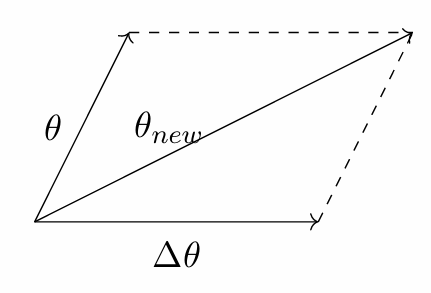
\includegraphics[scale=0.7]{image_1}
\end{figure}

Let us be a bit conservative: we move only by a small amount $\eta > 0$.

\begin{figure}[!htbp]
\centering
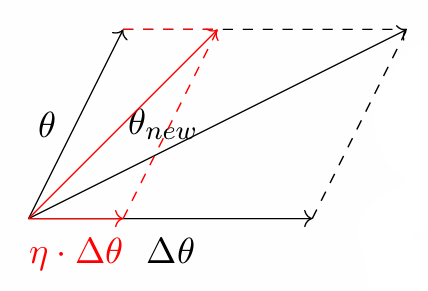
\includegraphics[scale=0.7]{image_2}
\end{figure}

$$i.e. \,\, \boldsymbol{\theta}_{new} = \boldsymbol{\theta} + \eta \cdot \Delta\boldsymbol{\theta}$$ \\[0.5em]

Now the question is what is the right $\Delta\boldsymbol{\theta}$ to use. The answer comes from Taylor Series.

\newpage

\subsection{Multivariate Taylor Series}

For a function $\mathcal{F}(\mathbf{x})$ expanded around $\mathbf{a} \in \mathbb{R}^n$, we have,

$$
\mathcal{F}(\mathbf{x}) = \mathcal{F}(\mathbf{a}) + (\mathbf{x} - \mathbf{a})' \nabla \mathcal{F}(\mathbf{a}) + \dfrac{1}{2!} (\mathbf{x} - \mathbf{a})' \nabla^2 \mathcal{F}(\mathbf{a}) (\mathbf{x} - \mathbf{a}) + \cdots
$$

\subsection{Derivation}

For ease of notation, take $\Delta \boldsymbol{\theta} = \boldsymbol{u}$. \\


With $\mathcal{F} = \mathscr{L}$(our Loss Function), $\mathbf{x} = \boldsymbol{\theta} + \eta \boldsymbol{u}$, $\mathbf{a} = \boldsymbol{\theta}$; from the Taylor Series we have,

\begin{align*}
\mathscr{L}(\boldsymbol{\theta} + \eta \boldsymbol{u}) &= \mathscr{L}(\boldsymbol{\theta}) + (\eta \boldsymbol{u})' \nabla \mathscr{L}(\boldsymbol{\theta}) + \dfrac{1}{2!} (\eta \boldsymbol{u})' \nabla^2 \mathscr{L}(\boldsymbol{\theta}) (\eta \boldsymbol{u}) + \cdots \\[0.5em]
&= \mathscr{L}(\boldsymbol{\theta}) + \eta \, \boldsymbol{u}' \nabla \mathscr{L}(\boldsymbol{\theta}) + \dfrac{\eta^2}{2!} \, \boldsymbol{u}' \nabla^2 \mathscr{L}(\boldsymbol{\theta}) \boldsymbol{u} + \cdots \\[0.5em]
&= \mathscr{L}(\boldsymbol{\theta}) + \eta \, \boldsymbol{u}' \nabla \mathscr{L}(\boldsymbol{\theta}) \left[ \eta \text{ typically being small } \eta^2, \eta^3, \ldots \rightarrow 0 \right]
\end{align*} 

Note that the move $\left( \eta \boldsymbol{u} \right)$ would be favourable only if,

$$\mathscr{L}(\boldsymbol{\theta} + \eta \boldsymbol{u}) - \mathscr{L}(\boldsymbol{\theta}) < 0$$

\textit{i.e.} if the new loss is less than the previous loss. \\

This implies $\boldsymbol{u}' \nabla \mathscr{L}(\boldsymbol{\theta}) < 0$, as $\eta$ is a positive quantity and more the negative $\boldsymbol{u}' \nabla \mathscr{L}(\boldsymbol{\theta})$ is, the more is favourable the move $\eta \boldsymbol{u}$. Now let us find out the range of $\boldsymbol{u}' \nabla \mathscr{L}(\boldsymbol{\theta})$. \\[0.5em]

$\bullet$ Let $\beta$ be the angle between $\boldsymbol{u}$ and $\nabla_{\boldsymbol{\theta}} \mathscr{L}(\boldsymbol{\theta})$, then we know that,
\[
-1 \leq \cos(\beta) = \dfrac{\boldsymbol{u}^T \nabla_{\boldsymbol{\theta}} \mathscr{L}(\boldsymbol{\theta})}{\|\boldsymbol{u}\| \cdot \|\nabla_{\boldsymbol{\theta}} \mathscr{L}(\boldsymbol{\theta})\|} \leq 1
\] \\[0.5em]

Multiplying throughout by $k = \|\boldsymbol{u}\| \cdot \|\nabla_{\boldsymbol{\theta}} \mathscr{L}(\boldsymbol{\theta})\|$:
\[
-k \leq k \cdot \cos(\beta) = \boldsymbol{u}^T \nabla_{\boldsymbol{\theta}} \mathscr{L}(\boldsymbol{\theta}) \leq k
\]

Thus,
\[
\mathscr{L}(\boldsymbol{\theta} + \eta \boldsymbol{u}) - \mathscr{L}(\boldsymbol{\theta}) = \boldsymbol{u}^T \nabla_{\boldsymbol{\theta}} \mathscr{L}(\boldsymbol{\theta}) = k \cdot \cos(\beta)
\]
will be most negative when $\cos(\beta) = -1$, \textit{i.e.}, when $\beta$ is $180^\circ$. \\[0.25em]

So our best move is at $180^{\circ}$ w.r.t. the gradient $\nabla \mathscr{L}(\boldsymbol{\theta})$.  In other words, we should move in a direction opposite to the gradient \textit{i.e.}

$$ \eta \Delta\boldsymbol{\theta} = - \eta \nabla \mathscr{L}(\boldsymbol{\theta})$$

The parameter update equations become

\begin{align} \label{eq:1}
w_{t+1} &= w_t - \eta \nabla w_t \nonumber \\
b_{t+1} &= b_t - \eta \nabla b_t
\end{align}

$$ \text{where, } \nabla w_t = \left. \dfrac{\partial \mathscr{L}(w, b)}{\partial w} \right|_{w = w_t,\, b = b_t}, \quad
\nabla b_t = \left. \dfrac{\partial \mathscr{L}(w, b)}{\partial b} \right|_{w = w_t,\, b = b_t} $$

\section{Batch / Vanilla Gradient Descent}

This is the simplest form of gradient descent with parameter update rules as in ~\ref{eq:1}. \\[0.15em]

\begin{algorithm}[H]
\caption{\texttt{gradient\_descent()}}
$t \leftarrow 0$\;
$max\_iterations \leftarrow 1000$\;

\While{$t < max\_iterations$}{
    $w_{t+1} \leftarrow w_t - \eta \, \nabla w_t$\;
    $b_{t+1} \leftarrow b_t - \eta \, \nabla b_t$\;
    $t \leftarrow t + 1$\;
}
\textbf{end}
\end{algorithm}



\begin{figure}[!htbp]
\centering
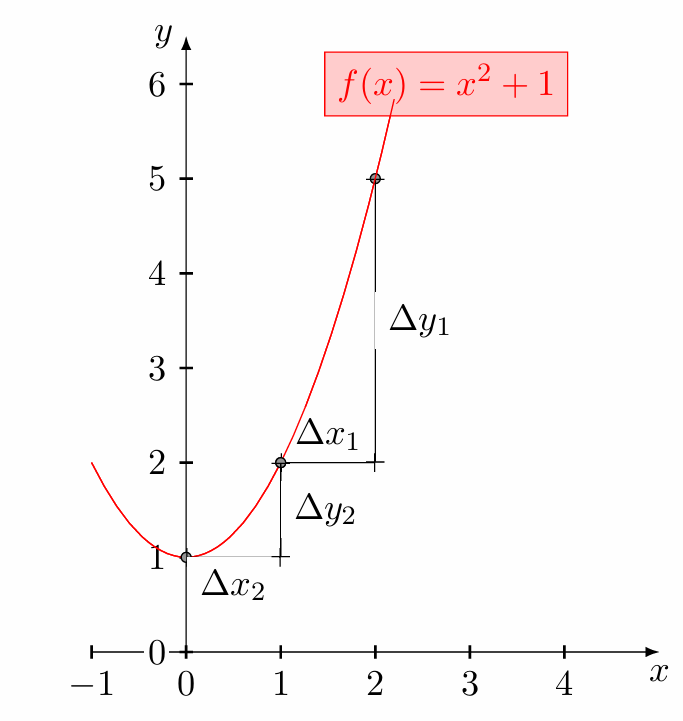
\includegraphics[scale=0.5]{image_3}
\end{figure}

\begin{itemize}
    \item When the curve is steep, the gradient $\left( \dfrac{\Delta y_1}{\Delta x_1} \right)$ is large.
    
    \item When the curve is gentle, the gradient $\left( \dfrac{\Delta y_2}{\Delta x_2} \right)$ is small.
    
    \item Recall that our weight updates are proportional to the gradient: $w_{new} = w - \eta \, \nabla w$
    
    \item Hence, in the areas where the curve is gentle the updates are small, whereas in the areas where the curve is steep the updates are large. That's why in gradient descent whenever the error surface is gentle we move slower and whenever it is steep we move faster.
\end{itemize}

The fact that it takes a lot of time to navigate regions having a gentle slope, gives 1 demerit point to Vanilla Gradient Descent. In the upcoming section we shall see that we can do better.


\begin{enumerate}
\item It’s called \textbf{batch} gradient descent because it uses the entire batch (full dataset) to compute each gradient.

\item It’s called \textbf{vanilla} gradient descent because it’s the simplest, unmodified form of gradient descent.
\end{enumerate}

\newpage

\section{Momentum Gradient Descent}


\end{document}